%-----------------------------------------------------------------------------%
\chapter{\babTiga}
%-----------------------------------------------------------------------------%
Penelitian ini bertujuan untuk mengevaluasi konfigurasi Hypervisor KVM yang disediakan secara default dalam konteks penggunaan \vm\ pada Apache Cloudstack. Tujuan utama adalah untuk memastikan bahwa \vm\ dapat mencapai kinerja yang optimal sesuai dengan spesifikasi sistem yang digunakan. Untuk mencapai tujuan ini, \saya\ akan melakukan penyesuaian konfigurasi atau tuning pada Hypervisor KVM dan kemudian membandingkannya dengan kondisi awal yang tidak mengalami tuning. Hasil pengujian akan dianalisis untuk menentukan apakah ada perbedaan signifikan dalam kinerja antara Hypervisor KVM yang telah dituning dengan yang belum dituning.

%-----------------------------------------------------------------------------%
\section{Tahapan Penelitian}
%-----------------------------------------------------------------------------%
\begin{figure}
    \centering
    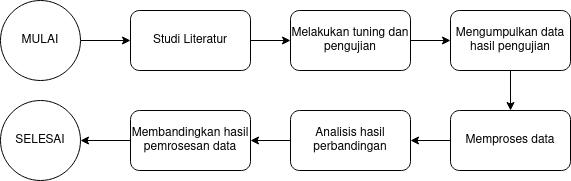
\includegraphics[width=1\textwidth]
    {assets/pics/tahapan-penelitian.png}
    \caption{Tahapan Penelitian}
    \label{fig:TahapanPenelitian}
\end{figure}

Penelitian ini akan dilakukan dalam beberapa tahap sesuai dengan diagram di gambar \ref{fig:TahapanPenelitian}. Tahap pertama melibatkan studi literatur untuk mengumpulkan semua informasi yang diperlukan. Studi literatur ini penting karena memberikan dasar pengetahuan yang kuat tentang topik yang akan diteliti, memungkinkan peneliti untuk memahami konteks dan kerangka kerja yang relevan.

Selanjutnya, penelitian melibatkan tuning terhadap Hypervisor KVM, dan pengujian dilakukan dengan tiga skenario, yaitu kompresi video, enkripsi data dengan AES, dan validasi integritas data menggunakan CRC32. Hasil dari pengujian ini akan memberikan gambaran mengenai konfigurasi yang paling optimal dan sesuai, serta membantu dalam pemahaman lebih lanjut tentang pengaruh tuning terhadap performa Hypervisor KVM.

%-----------------------------------------------------------------------------%
\section{Persiapan Lingkungan untuk Pengujian dan Analisis}
%-----------------------------------------------------------------------------%
\begin{figure}
    \centering
    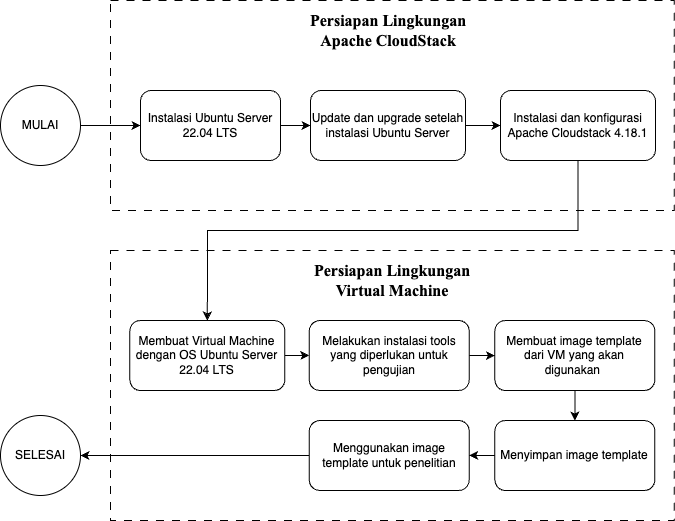
\includegraphics[width=1\textwidth]
    {assets/pics/persiapan_lingkungan_penelitian.png}
    \caption{Persiapan Lingkungan Penelitian}
    \label{fig:PersiapanLingkunganPenelitian}
\end{figure}


Proses persiapan lingkungan untuk pengujian dan analisis yang tergambar dalam gambar \ref{fig:PersiapanLingkunganPenelitian} menggambarkan serangkaian langkah sistematis yang penting untuk memastikan integritas hasil penelitian. Proses ini dimulai dengan tahap inisiasi yang meliputi instalasi Ubuntu Server 22.04 LTS, sebuah sistem operasi yang stabil dan sering digunakan untuk keperluan server. Instalasi ini menjadi landasan dasar bagi infrastruktur yang akan dikembangkan.

Setelah sistem operasi terinstal, dilakukan pembaruan dan peningkatan sistem operasi tersebut untuk memastikan semua komponen sistem berada pada versi terkini serta keamanan sistem terjaga. Langkah ini krusial untuk menutup potensi kerentanan yang mungkin ada pada sistem. Selanjutnya, Apache Cloudstack versi 4.18.1 diinstal dan dikonfigurasikan. Apache Cloudstack berfungsi sebagai platform manajemen cloud yang memungkinkan pembuatan dan pengelolaan infrastruktur cloud yang kompleks, yang merupakan elemen kunci dalam penelitian ini.

Dalam pembuatan lingkungan virtual, dibuat \vm\ yang menggunakan sistem operasi yang sama, yaitu Ubuntu Server 22.04 LTS. Pembuatan VM ini memungkinkan simulasi berbagai skenario penelitian dalam lingkungan yang terisolasi. Selanjutnya, untuk keperluan analisis dan pengujian, berbagai perangkat lunak yang akan digunakan untuk melakukan pengujian akan di install.

Tahapan selanjutnya merupakan pembuatan image template dari VM yang telah dikonfigurasikan. Proses ini memungkinkan duplikasi VM dengan cepat dan efisien untuk pengujian berulang atau skenario analisis yang berbeda, menjamin konsistensi lingkungan penelitian. Image template ini kemudian digunakan sebagai standar untuk penelitian lebih lanjut, memastikan bahwa setiap VM yang dibuat untuk tujuan pengujian memiliki konfigurasi yang identik.

Setelah semua dilakukan hal ini menandakan bahwa lingkungan penelitian telah siap untuk diuji dan dianalisis. Kesiapan lingkungan ini esensial untuk memastikan bahwa pengujian yang dilakukan dapat diulang dengan cepat dan efisien.

%-----------------------------------------------------------------------------%
\subsection{Instalasi dan Konfigurasi Apache Cloudstack}
%-----------------------------------------------------------------------------%
Dalam instalasi ini \saya\ akan menggunakan \f{Home Network} di IP 192.168.0.0/24. Pertama \saya\ akan melakukan instalasi \f{tools} yang dibutuhkan dengan perintah:

\begin{listing}[H]
    \begin{minted}{bash}
    $ sudo apt-get install -y openntpd openssh-server vim htop tar
    $ sudo apt-get install -y intel-microcode
    \end{minted}
\end{listing}

Perintah ini akan menginstall \f{tools} openntpd, openssh-server, vim, htop, tar, dan intel-microcode. Setelah melakukan instalasi \f{tools} ini kemudian \saya\ akan mengganti password dari user root dengan perintah:

\begin{listing}[H]
    \begin{minted}{bash}
    $ sudo passwd root
    \end{minted}
\end{listing}

Password root user ini nantinya akan digunakan untuk memastikan bahwa Apache CloudStack dapat mengakses komputer host untuk melakukan provisioning \vm dan operasi lainnya.
%-----------------------------------------------------------------------------%
\subsubsection{Pengaturan Jaringan}
%-----------------------------------------------------------------------------%
\saya\ melakukan pengaturan \f{Linux Bridge} yang akan menghandle jaringan CloudStack \f{public, guest, management} dan \f{storage}. Untuk penyederhanaan \saya\ akan menggunakan satu \f{bridge} yang bernama \textbf{cloudbr0} yang akan digunakan untuk semua jaringan ini. Untuk menginstall \f{tools} yang diperlukan untuk membuat \f{bridge} digunakan perintah:

\begin{listing}[H]
    \begin{minted}{bash}      
    $ sudo apt-get install bridge-utils
    \end{minted}
\end{listing}

Setelah menginstall \f{tools} ini, \saya\ akan mengkonfigurasi \f{bridge} \textbf{cloudbr0} dengan menggunakan netplan. Pertama \saya\ memastikan bahwa seleuruh konfigurasi netplan sekarang di rename dengan menambahkan extensi \textbf{.bak} sebagai backup. Setelah itu \saya\ membuat file konfigruasi netplan dengan perintah:

\begin{listing}[H]
    \begin{minted}{bash}     
    $ sudo nano /etc/netplan/01-netcfg.yaml
    \end{minted}
\end{listing}

Perintah ini akan membuka text editor nano dengan file \texttt{01-netcfg.yaml}. Kemudian \saya\ mengisi file konfigurasi tersebut dengan konfigurasi yang terlihat di kode \ref{code:netplan_config}:

\begin{listing}[H]
    \begin{minted}{yaml}
    network:
        version: 2
        renderer: networkd
        ethernets:
            enp2s0:
                dhcp4: false
                dhcp6: false
                optional: true
        bridges:
            cloudbr0:
                addresses: [192.168.0.10/24]
                routes:
                -   to: default
                    via: 192.168.0.1
                nameservers:
                    addresses: [1.1.1.1,8.8.8.8]
                interfaces: [enp2s0]
                dhcp4: false
                dhcp6: false
                parameters:
                    stp: false
                    forward-delay: 0
    \end{minted}
    \caption{Konfigurasi Netplan untuk Cloudbr0}
    \label{code:netplan_config}
\end{listing}

Dalam konfigurasi ini IP dari \f{bridge} \textbf{cloudbr0} adalah 192.168.0.10/24 dan akan menggunakan DNS 1.1.1.1 dan 8.8.8.8. Setelah melakukan konfigurasi ini \saya\ akan mengaktifkan \f{bridge} \textbf{cloudbr0} dengan perintah:

\begin{listing}[H]
    \begin{minted}{bash}     
    $ sudo netplan generate
    $ sudo netplan apply
    $ sudo reboot
    \end{minted}
\end{listing}

Dengan perintah ini akan dilakukan netplan generate dan apply, setelah itu sistem akan melakukan reboot. Sampai sini pembuatan \f{bridge} \textbf{cloudbr0} sudah selesai.

\subsubsection{Instalasi Cloudstack}
Pertama \saya\ akan melakukan instalasi \texttt{cloudstack-management} dan juga \texttt{mysql-server}. Database yang akan digunakan untuk Apache CloudStack dalam penelitian ini adalah MySQL.

\begin{listing}[H]
    \begin{minted}{bash}    
    $ sudo mkdir -p /etc/apt/keyrings
    $ wget -O- http://packages.shapeblue.com/release.asc | gpg --dearmor | sudo tee /etc/apt/keyrings/cloudstack.gpg > /dev/null
    
    $ echo deb [signed-by=/etc/apt/keyrings/cloudstack.gpg] http://packages.shapeblue.com/cloudstack/upstream/debian/4.18 / > /etc/apt/sources.list.d/cloudstack.list \\
    $ sudo apt-get update -y
    $ sudo apt-get install cloudstack-management mysql-server
    \end{minted}
\end{listing}

Perintah tersebut digunakan untuk menginstal \f{CloudStack Management Server} versi 4.18 dan MySQL Server. Pertama, perintah akan membuat direktori untuk menyimpan kunci GPG yang digunakan untuk mengotentikasi paket dari repositori CloudStack. Kemudian, kunci GPG tersebut diunduh, didekompresi, dan disimpan dalam direktori yang telah dibuat. Selanjutnya, konfigurasi ditambahkan ke file \texttt{sources.list.d} untuk menandatangani paket-paket dari repositori CloudStack. Setelah itu, daftar paket diperbarui dan \f{CloudStack Management Server} serta MySQL Server diinstal menggunakan perintah apt-get. Selain ini juga akan dilakukan instalasi \f{tools} cloudstack usage dan billing, dengan menggunakan perintah:

\begin{listing}[H]
    \begin{minted}{bash}  
    $ sudo apt-get install cloudstack-usage
    \end{minted}
\end{listing}

\subsubsection{Konfigurasi Database}
Setelah MySQL server selesai di install \saya\ akan melakukan konfigurasi setting InnoDB di mysql server dengan perintah:

\begin{listing}[H]
    \begin{minted}{bash}      
    $ sudo nano /etc/mysql/mysql.conf.d/mysqld.cnf
    \end{minted}
\end{listing}

Kemudian \saya\ menghapus seluruh isi dari file tersebut dan menggantinya dengan konfigurasi yang terlihat di kode \ref{code:mysql_config}:

\begin{listing}[H]
    \begin{minted}{ini}
    [mysqld]

    server_id = 1
    sql-mode="STRICT_TRANS_TABLES,NO_ENGINE_SUBSTITUTION,ERROR_FOR_DIVISION_BY_ZERO
    NO_ZERO_DATE,NO_ZERO_IN_DATE,NO_ENGINE_SUBSTITUTION"
    innodb_rollback_on_timeout=1
    innodb_lock_wait_timeout=600
    max_connections=1000
    log-bin=mysql-bin
    binlog-format = 'ROW'
    \end{minted}
    \caption{Konfigurasi mysqld.cnf}
    \label{code:mysql_config}
\end{listing}

Setelah selesai melakukan konfigurasi \saya\ merestart MySQL server. Hal ini dilakukan agar mysql menggunakan setting yang terbaru. Untuk melakukan restart MySQL server \saya\ menggunakan perintah:

\begin{listing}[H]
    \begin{minted}{bash}     
    $ systemctl restart mysql
    \end{minted}
\end{listing}

Setelah MySQL server selesai di restart langkah selanjunya adalah melakukan deploy database untuk CloudStack. Deploy server ini harus dilakukan sebagai user root. Deploy dilakukan dengan perintah:

\begin{listing}[H]
    \begin{minted}{bash}       
    $ sudo cloudstack-setup-databases cloud:cloud@localhost --deploy-as=root:password -i 192.168.0.10
    \end{minted}
\end{listing}

IP yang digunakan \saya\ adalah IP dari sistem host.

\subsubsection{Konfigurasi Storage}
Pada tahap ini \saya\ akan melakukan konfigurasi untuk penyimpanan dari cloudstack. Pertama akan dilakukan instalasi storage driver yang akan digunakan dengan perintah:

\begin{listing}[H]
    \begin{minted}{bash}       
    $ sudo apt-get install nfs-kernel-server quota
    $ echo "/export  *(rw,async,no_root_squash,no_subtree_check)" > /etc/exports
    $ sudo mkdir -p /export/primary /export/secondary
    $ sudo exportfs -a
    \end{minted}
\end{listing}

Perintah \texttt{sudo apt-get install nfs-kernel-server quota} digunakan untuk menginstal perangkat lunak server NFS dan modul Quota pada sistem Linux. Selanjutnya, perintah \texttt{echo "/export *(rw,async,no\_root\_squash,no\_subtree\_check)" > /etc/exports} digunakan untuk menetapkan konfigurasi eksport NFS dengan opsi akses tertentu. Kemudian, perintah \texttt{sudo mkdir -p /export/primary /export/secondary} membuat direktori yang akan diakses oleh klien NFS. Terakhir, perintah \texttt{sudo exportfs -a} mengekspor semua direktori yang telah dikonfigurasi sebelumnya untuk diakses oleh klien NFS. Dengan demikian, rangkaian perintah ini mempersiapkan server NFS untuk berbagi data melalui jaringan. Setelah itu \saya\ melakukan konfigurasi NFS server dengan perintah:

\begin{listing}[H]
    \begin{minted}{bash} 
    $ sed -i -e 's/^RPCMOUNTDOPTS="--manage-gids"$/RPCMOUNTDOPTS="-p 892 --manage-gids"/g' /etc/default/nfs-kernel-server
    $ sed -i -e 's/^STATDOPTS=$/STATDOPTS="--port 662 --outgoing-port 2020"/g' /etc/default/nfs-common
    $ echo "NEED_STATD=yes" >> /etc/default/nfs-common
    $ sed -i -e 's/^RPCRQUOTADOPTS=$/RPCRQUOTADOPTS="-p 875"/g' /etc/default/quota
    $ service nfs-kernel-server restart
    \end{minted}
\end{listing}

Perintah-perintah tersebut digunakan untuk mengubah konfigurasi pada server NFS dan Quota pada sistem Linux. Pertama, menggunakan \texttt{sed}, konfigurasi NFS Mount Daemon dan NFS Stat Daemon diubah untuk menggunakan port yang ditentukan dan mengaktifkan manajemen GID. Selanjutnya, sistem Stat Daemon diaktifkan dengan menambahkan opsi yang sesuai ke file konfigurasi NFS Common. Kemudian, konfigurasi RPC Quota Daemon diubah untuk menggunakan port yang ditentukan. Terakhir, layanan NFS Kernel Server di-restart untuk menerapkan perubahan konfigurasi yang telah dilakukan.

\subsubsection{Konfigurasi KVM}
Tahap selanjutnya adalah konfigurasi KVM dan cloudstack agent. Pertama \saya\ melakukan install KVM dan CloudStack agent dengan perintah:

\begin{listing}[H]
    \begin{minted}{bash}       
    $ sudo apt-get install qemu-kvm cloudstack-agent
    \end{minted}
\end{listing}

Setelah KVM dan CloudStack agent terinstall \saya\ akan melakukan konfigurasi KVM. Pertama \saya\ akan mengubah konfigurasi \texttt{libvirt} dengan perintah:

\begin{listing}[H]
    \begin{minted}{bash}       
    $ sudo sed -i -e 's/\#vnc_listen.*$/vnc_listen = "0.0.0.0"/g' /etc/libvirt/qemu.conf
    $ sudo echo LIBVIRTD_ARGS=\"--listen\" >> /etc/default/libvirtd
    $ sudo systemctl mask libvirtd.socket libvirtd-ro.socket libvirtd-admin.socket libvirtd-tls.socket libvirtd-tcp.socket
    $ sudo systemctl restart libvirtd
    \end{minted}
\end{listing}

Perintah tersebut digunakan untuk mengkonfigurasi \texttt{libvirt}, sebuah toolkit untuk mengelola virtualisasi di Linux. Pertama, perintah \texttt{sed} digunakan untuk mengubah pengaturan dalam file konfigurasi \texttt{qemu.conf} agar libvirt dapat menerima koneksi VNC dari semua interface jaringan. Kemudian, argumen \texttt{--listen} ditambahkan ke konfigurasi libvirtd melalui file \texttt{/etc/default/libvirtd}, yang membuat libvirt mendengarkan koneksi dari interface jaringan. Selanjutnya, perintah \texttt{systemctl mask} digunakan untuk menonaktifkan unit-unit systemd yang terkait dengan libvirtd, seperti socket-soket yang tidak diperlukan, untuk menghindari penggunaan yang tidak diinginkan. Terakhir, layanan libvirtd di-restart agar perubahan konfigurasi dapat diterapkan.

Selanjutnya \saya\ melakukan konfigurasi default untuk libvirtd dengan perintah:

\begin{listing}[H]
    \begin{minted}{bash}
    $ echo 'listen_tls=0' >> /etc/libvirt/libvirtd.conf
    $ echo 'listen_tcp=1' >> /etc/libvirt/libvirtd.conf
    $ echo 'tcp_port = "16509"' >> /etc/libvirt/libvirtd.conf
    $ echo 'mdns_adv = 0' >> /etc/libvirt/libvirtd.conf
    $ echo 'auth_tcp = "none"' >> /etc/libvirt/libvirtd.conf
    $ systemctl restart libvirtd
    \end{minted}
\end{listing}

Perintah-perintah tersebut digunakan untuk mengkonfigurasi default pada file konfigurasi libvirt (libvirtd.conf). Pertama, dengan menambahkan \texttt{listen\_tls=0}, libvirt diminta untuk tidak mendengarkan koneksi TLS, sehingga mematikan mode tersebut. Kemudian, \texttt{listen\_tcp=1} mengaktifkan libvirt untuk mendengarkan koneksi TCP/IP. Penambahan \texttt{tcp\_port = "16509"} menetapkan port TCP yang akan digunakan oleh libvirt. Selanjutnya, dengan \texttt{mdns\_adv = 0}, mDNS advertise untuk penemuan otomatis layanan libvirt dimatikan. Terakhir, \texttt{auth\_tcp = "none"} mengatur libvirt untuk menerima koneksi TCP/IP tanpa melakukan otentikasi. Setelah perubahan-perubahan ini diterapkan, layanan libvirt di-restart agar konfigurasi baru dapat mulai digunakan. Konfigurasi default ini hanya diperlukan \saya\ saat setup awal, karena saat menambahkan host KVM dalam CloudStack, konfigurasi yang lebih aman menggunakan TLS akan diterapkan secara otomatis.

Kemudian \saya\ menambahkan konfigurasi berikut ini di \texttt{/etc/sysctl.conf} lalu menjalankan \texttt{sysctl -p}. Konfigurasi ini perlu ditambahkan pada host tertentu ditempat menjalankan docker dan service lainnya.

\begin{listing}[H]
    \begin{minted}{bash}       
    $ nano /etc/sysctl.conf
    $ echo 'net.bridge.bridge-nf-call-arptables = 0' >> /etc/sysctl.conf
    $ echo 'net.bridge.bridge-nf-call-iptables = 0' >> /etc/sysctl.conf
    $ sysctl -p
    \end{minted}
\end{listing}

Pad perintah ini pertama, akan dibuka file \texttt{/etc/sysctl.conf} menggunakan teks editor nano. Kemudian, dengan menambahkan baris \texttt{net.bridge.bridge-nf-call-arptables = 0} dan \texttt{net.bridge.bridge-nf-call-iptables = 0} ke dalam file tersebut, Ini akan mematikan fungsi kernel yang biasanya dipanggil saat menggunakan Docker dan jembatan jaringan (bridge). Ini penting karena beberapa layanan, seperti Docker, kadang memerlukan konfigurasi khusus agar berjalan dengan lancar di lingkungan host. Terakhir, dengan menjalankan perintah \texttt{sysctl -p}, perubahan konfigurasi yang telah dibuat akan diterapkan tanpa harus me-reboot sistem, sehingga memungkinkan kernel untuk memuat ulang konfigurasi yang baru diterapkan.

Setelah itu \saya\ akan mengenerate host id dengan uuid, hal ini dapat dilakukan dengan perintah:

\begin{listing}[H]
    \begin{minted}{bash}   
    $ sudo apt-get install uuid
    $ UUID=$(uuid)
    $ echo host_uuid = \"$UUID\" >> /etc/libvirt/libvirtd.conf
    $ systemctl restart libvirtd
    \end{minted}
\end{listing}

Perintah ini digunakan untuk meng-generate UUID \f{(Universally Unique Identifier)} untuk host dan mengintegrasikannya ke dalam konfigurasi \texttt{libvirtd}. Perintah \texttt{UUID=\$(uuid)} digunakan untuk meng-generate UUID secara acak dan menyimpannya dalam variabel \texttt{UUID}. UUID adalah string panjang yang unik secara global dan digunakan untuk mengidentifikasi entitas secara unik di sistem. Kemudian, perintah \texttt{echo host\_uuid = \" \$UUID \"  >> /etc/libvirt/libvirtd.conf} menambahkan baris \texttt{host\_uuid = "<nilai UUID>"} ke dalam file konfigurasi \texttt{libvirtd.conf}. Fungsi baris ini adalah untuk menyimpan UUID host di konfigurasi \texttt{libvirtd}, yang akan digunakan oleh \texttt{libvirt} untuk mengidentifikasi host secara unik dalam lingkungan virtualisasi. Terakhir, perintah \texttt{systemctl restart libvirtd} digunakan untuk merestart layanan libvirtd agar perubahan konfigurasi yang telah dilakukan dapat diterapkan.

\subsubsection{Konfigurasi Firewall}
Untuk melakukan konfigruasi firewall \saya\ menggunakan perintah:

\begin{listing}[H]
    \begin{minted}{bash}       
    # configure firewall rules to allow useful ports
    $ NETWORK=192.168.0.0/24
    $ iptables -A INPUT -s $NETWORK -m state --state NEW -p udp --dport 111 -j ACCEPT
    $ iptables -A INPUT -s $NETWORK -m state --state NEW -p tcp --dport 111 -j ACCEPT
    $ iptables -A INPUT -s $NETWORK -m state --state NEW -p tcp --dport 2049 -j ACCEPT
    $ iptables -A INPUT -s $NETWORK -m state --state NEW -p tcp --dport 32803 -j ACCEPT
    $ iptables -A INPUT -s $NETWORK -m state --state NEW -p udp --dport 32769 -j ACCEPT
    $ iptables -A INPUT -s $NETWORK -m state --state NEW -p tcp --dport 892 -j ACCEPT
    $ iptables -A INPUT -s $NETWORK -m state --state NEW -p tcp --dport 875 -j ACCEPT
    $ iptables -A INPUT -s $NETWORK -m state --state NEW -p tcp --dport 662 -j ACCEPT
    $ iptables -A INPUT -s $NETWORK -m state --state NEW -p tcp --dport 8250 -j ACCEPT
    $ iptables -A INPUT -s $NETWORK -m state --state NEW -p tcp --dport 8080 -j ACCEPT
    $ iptables -A INPUT -s $NETWORK -m state --state NEW -p tcp --dport 9090 -j ACCEPT
    $ iptables -A INPUT -s $NETWORK -m state --state NEW -p tcp --dport 16514 -j ACCEPT
    
    $ sudo apt-get install iptables-persistent
    \end{minted}
\end{listing}

Perintah tersebut bertujuan untuk mengonfigurasi aturan firewall pada sistem menggunakan iptables, dengan fokus pada pembukaan port-port yang umum digunakan untuk layanan-layanan yang digunakan. Pertama, baris \texttt{NETWORK=192.168.0.0/24} mendefinisikan jaringan yang diizinkan melalui aturan firewall. Selanjutnya, setiap perintah \texttt{iptables -A INPUT ... -j ACCEPT} menambahkan aturan iptables untuk mengizinkan koneksi baru pada port tertentu dari jaringan yang telah ditentukan sebelumnya. Misalnya, perintah \texttt{iptables -A INPUT -s \$NETWORK -m state --state NEW -p udp --dport 111 -j ACCEPT} mengizinkan koneksi UDP baru pada port 111 dari jaringan yang telah ditentukan.

Aturan-aturan tersebut dirancang untuk membuka akses ke port-port yang umum digunakan oleh layanan-layanan seperti NFS, RPC, dan layanan manajemen tertentu. Setelah semua aturan ditambahkan, perintah \texttt{apt-get install iptables-persistent} digunakan untuk menginstal paket \texttt{iptables-persistent}, yang bertujuan agar konfigurasi aturan firewall yang telah dibuat akan dipertahankan dan diterapkan secara otomatis setiap kali sistem di-boot. Dengan demikian, langkah-langkah ini membantu menjaga keamanan sistem dengan memperbolehkan akses hanya ke port-port yang diperlukan dan memastikan bahwa aturan firewall tidak hilang setelah reboot.

Setelah itu kita harus menonaktifkan \texttt{apparmor} pada \texttt{libvirtd}, dikarenakan CloudStack melakukan berbagai macam hal yang memungkinkan bisa terblokir oleh mekanisme pertahanan seperti \texttt{apparmor} \cite{apacheHostInstallation}. Untuk mematikan apparmor \saya\ melakukan perintah:

\begin{listing}[H]
    \begin{minted}{bash}   
    $ ln -s /etc/apparmor.d/usr.sbin.libvirtd /etc/apparmor.d/disable/
    $ ln -s /etc/apparmor.d/usr.lib.libvirt.virt-aa-helper /etc/apparmor.d/disable/
    $ apparmor_parser -R /etc/apparmor.d/usr.sbin.libvirtd
    $ apparmor_parser -R /etc/apparmor.d/usr.lib.libvirt.virt-aa-helper
    \end{minted}
\end{listing}

Perintah-perintah tersebut bertujuan untuk menonaktifkan \texttt{apparmor} pada layanan \texttt{libvirtd} (Libvirt daemon). Langkah pertama adalah membuat symlink (tautan simbolis) dari file konfigurasi \texttt{apparmor} yang berkaitan dengan \texttt{libvirtd} dan helpernya ke dalam direktori \texttt{/etc/apparmor.d/disable/}. Dengan melakukan ini, \texttt{apparmor} diarahkan untuk mengabaikan atau menonaktifkan aturan-aturan yang telah didefinisikan untuk \texttt{libvirtd}. Selanjutnya, perintah \texttt{apparmor\_parser -R} digunakan untuk me-refresh aturan-aturan \texttt{apparmor} yang terkait dengan \texttt{libvirtd} dan helpernya, sehingga aturan-aturan yang telah dinonaktifkan dengan symlink dapat diaplikasikan secara efektif.

Perlu \saya\ ingat bahwa menonaktifkan \texttt{apparmor} dapat meningkatkan risiko keamanan sistem karena menghilangkan lapisan proteksi yang diberikan oleh \texttt{apparmor} terhadap layanan tersebut.

\subsubsection{Menjalankan CloudStack}
Sampai tahap ini instalasi CloudStack sudah selesai dan untuk menjalankan CloudStack \saya\ menggunakan perintah ini:

\begin{listing}[H]
    \begin{minted}{bash}  
    $ sudo cloudstack-setup-management
    \end{minted}
\end{listing}

Setelah server manajemen sudah UP, CloudStack dapat \saya\ akses di \texttt{http://192.168.0.10:8080} (IP dari \textbf{cloudbr0}) dan masuk dengan kredensial default yaitu admin/admin. Saat masuk pertama kali akan dilanjutkan dengan pengaturan Apache CloudStack. Dikonfigurasi \saya\ akan mengatur Zone, Network, Pod, Cluster, Host, Primary Storage, dan Secondary Storage.

\begin{figure}
    \centering
    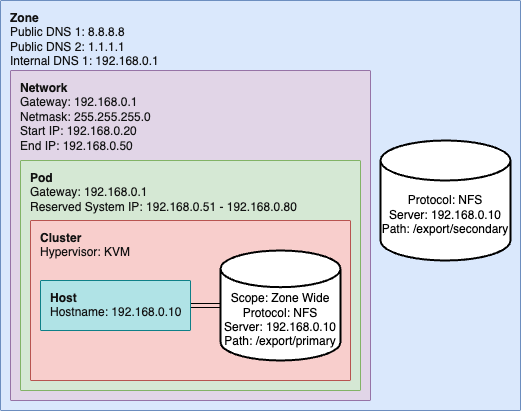
\includegraphics[width=1\textwidth]
    {assets/pics/cloudstack_config.png}
    \caption{Konfigurasi Apache CloudStack}
    \label{fig:KonfigurasiApacheCloudStack}
\end{figure}

% Pada gambar \ref{fig:KonfigurasiApacheCloudStack} adalah konfigurasi Apache CloudStack yang dilakukan oleh \saya\. Pada Zone \saya\ menggunakan public DNS \texttt{8.8.8.8} dan 1.1.1.1, DNS ini adalah DNS publik milik Google dan Cloudflare, dan untuk internal DNSnya \saya\ menggunakan IP \texttt{192.168.0.1} IP ini adalah IP dari gateway di jaringan \f{Home Network} \saya\. Untuk Network \saya\ menggunakan IP \texttt{192.168.0.1} untuk gateway yang akan mengarahkan seluruh traffic dari CloudStack ke jaringan \f{Home Network} \saya\ dan untuk Netmask \saya\ menggunakan \texttt{255.255.255.0} yang merupakan netmask dari jaringan \f{Home Network} \saya\. Hal ini menandakan bahwa ada sebanyak 254 IP yang bisa digunakan dalam jaringan \f{Home Network} \saya\ untuk CloudStack. Untuk range IP di network di set di \texttt{192.168.0.20} sampai \texttt{192.168.0.50}, ini berarti ada sebanyak 30 IP yang bisa digunakan oleh \vm\ yang akan dibuat. Untuk Pod \saya\ menggunakan IP \texttt{192.168.0.1} untuk gatewaynya dan untuk \f{Reserved System IP} \saya\ menggunaklan IP range \texttt{192.168.0.51} sampai \texttt{192.168.0.80}. Untuk Cluster \saya\ menggunakan KVM sebagai Hypervisor dan untuk Host \saya\ menggunakan IP \texttt{192.168.0.10}, ini adalah IP dari host yang akan digunakan oleh CloudStack. Untuk Primary Storage \saya\ menggunakan protokol NFS dengan scope Zone Wide di server \texttt{192.168.0.10} di path \texttt{/export/primary}. dan untuk Secondary Storage \saya\ protokol NFS di server \texttt{192.168.90.10} di path \texttt{/export/secondary}.

Pada gambar \ref{fig:KonfigurasiApacheCloudStack}, terlihat konfigurasi Apache CloudStack yang \saya\ terapkan. Pada Zone, \saya\ menggunakan public DNS yaitu \texttt{8.8.8.8} dan \texttt{1.1.1.1}, yang merupakan DNS publik dari Google dan Cloudflare. Sementara untuk DNS internal, \saya\ menggunakan IP \texttt{192.168.0.1} yang merupakan IP gateway di jaringan Home Network. Untuk Network, \saya\ menetapkan IP \texttt{192.168.0.1} sebagai gateway untuk mengarahkan seluruh traffic dari CloudStack ke jaringan \f{Home Network} \saya. Netmask yang \saya\ gunakan adalah \texttt{255.255.255.0}, dimana memiliki total IP yang dapat dipakai hingga 254 IP dalam jaringan \f{Home Network} untuk CloudStack.

Rentang IP di Network \saya\ tetapkan dari \texttt{192.168.0.20} hingga \texttt{192.168.0.50}, yang artinya terdapat 30 IP yang tersedia untuk VM yang akan dibuat. Pada Pod, \saya\ menggunakan IP \texttt{192.168.0.1} sebagai gateway dan \f{Reserved System IP} dari \texttt{192.168.0.51} hingga \texttt{192.168.0.80}. \f{Reserved System IP} ini merupakan sistem yang dibuat oleh CloudStack secara otomatis yang menjalankan fungsi seperti manajemen jaringan, \f{load balancing}, dan lain-lain. Pada Cluster, \saya\ menggunakan KVM sebagai Hypervisor dengan Host IP di \texttt{192.168.0.10}, yang merupakan IP dari host yang akan digunakan oleh CloudStack.

Untuk Primary Storage, \saya\ menggunakan protokol NFS dengan cakupan Zone Wide pada server \texttt{192.168.0.10} dan path \texttt{/export/primary}, yang mana Primary Storage adalah penyimpanan yang nanti akan digunakan untuk operasi \vm\ secara langsung. Sedangkan untuk Secondary Storage, \saya\ menggunakan protokol NFS pada server \texttt{192.168.90.10} dengan path \texttt{/export/secondary}, yang mana Secondary Storage adalah penyimpanan yang digunakan untuk menyimpan data yang jarang diakses secara langsung oleh \vm\ ataupun sistem dari CloudStack.

Setelah konfigurasi selesai, \saya\ melihat data di \texttt{Navigation>Infrasturcture>Summary} dan memastikan seluruh komponen sudah dinyalakan. Untuk langkah selanjutnya \saya\ akan menambahkan file iso yang diinginkan untuk membuat instance.

%-----------------------------------------------------------------------------%
\subsection{Persiapan \vm}
%-----------------------------------------------------------------------------%
Pada tahap ini akan dijelaskan bagaimana cara \saya\ membuat \vm\ yang akan digunakan untuk melakukan pengujian. \vm\ yang akan dibuat menggunakan image Ubuntu Server 22.04 LTS yang telah diinstal sebelumnya.

%-----------------------------------------------------------------------------%
\subsubsection{Image Ubuntu Server 22.04 LTS}
%-----------------------------------------------------------------------------%
Langkah pertama yang \saya\ lakukan adalah mengunduh file image ISO Ubuntu Server 22.04 LTS dari situs resmi Ubuntu dan menyimpannya di sistem host. Agar dapat digunakan oleh CloudStack, file ISO ini perlu di-hosting agar dapat diakses melalui alamat IP host. Hosting ini akan dilakukan menggunakan Apache2, sebuah aplikasi web server. Setelah konfigurasi Apache2 selesai dan file image ISO dapat diakses melalui alamat IP, selanjutnya \saya\ membuka CloudStack dan menuju ke \texttt{Configuration>Global Settings>All Settings}. Di sini, \saya\ akan mengisi konfigurasi \texttt{"Secstorage allow internal sites"} dengan nilai \texttt{192.168.0.0/24} (Home network) dan menyimpan pengaturan tersebut. Setelah itu, \saya\ pergi ke \texttt{Images>ISOs} dan memilih opsi "register ISO". Kemudian \saya\ menambahkan file ISO Ubuntu Server 22.04 LTS yang telah diunduh sebelumnya dengan memasukkan alamat URL image ISO dari sistem host.

%-----------------------------------------------------------------------------%
\subsubsection{Membuat Image Template}
%-----------------------------------------------------------------------------%
Setelah ISO image sudah siap digunakan langkah selanjutnya yang \saya\ lakukan adalah membuat image template dengan pergi ke \texttt{Compute>Instances} dan memilih "Add Instances". Konfigurasi \vm\ yang digunakan \saya\ adalah seperti ini:

\begin{enumerate}
    \item Deployment Infrastructure
          \begin{itemize}
              \item Pod: Default
              \item Cluster: Default
              \item Host: Default
          \end{itemize}

    \item Template/ISO

          ISO Ubuntu Server 22.04 LTS

    \item Compute Offering

          \saya\ memilih tipe High Instance dengan spesifikasi:
          \begin{itemize}
              \item CPU: 4 vCPU
              \item Clock Speed: 2.0 GHz
              \item Memory: 4096 MB
          \end{itemize}

    \item Data Disk

          Pada penelitian ini \vm\ akan diberikan data disk berukuran 20GB.

    \item Networks

          Di bagian jaringan, \saya\ membuat jaringan baru untuk digunakan oleh \vm\ dengan menggunakan template \texttt{"Network Offering used for CloudStack Kubernetes Service"} dan mengatur Gateway menjadi \texttt{192.168.0.1} (Gateway Home Network) serta Netmask menjadi \texttt{255.255.255.0}. Untuk DNS 1, \saya\ menggunakan \texttt{1.1.1.1} (Cloudflare DNS), dan untuk DNS 2, \saya\ menggunakan \texttt{8.8.8.8} (Google DNS).
\end{enumerate}

Setelah instance siap digunakan, \saya\ membuka konsol dari instance dan melakukan instalasi standar Ubuntu Server 22.04 LTS. Setelah instalasi Ubuntu Server selesai, \saya\ melanjutkan dengan instalasi program-program yang akan digunakan untuk penelitian. Program-program yang digunakan termasuk \texttt{ffmpeg} untuk melakukan kompresi video, \texttt{python} untuk melakukan benchmark enkripsi, dekripsi, dan validasi integritas data.

Setelah selesai menginstal semua program yang diperlukan, langkah berikutnya yang dilakukan \saya\ adalah membuat image template dari \vm\ yang baru dibuat dengan cara pergi ke \texttt{Storage>Volumes} dan memilih opsi \texttt{Create template from volume}. Template ini akan sangat berguna untuk memudahkan pembuatan \vm\ baru dengan konfigurasi dan aplikasi yang sudah disiapkan jika terjadi masalah atau jika dibutuhkan pembuatan \vm\ baru.

%-----------------------------------------------------------------------------%
\section{Tuning Hypervisor KVM}
%-----------------------------------------------------------------------------%
Untuk melakukan tuning pada Hypervisor KVM, \saya\ menggunakan tools virsh, sebuah command line tool yang disediakan oleh virtualization API libvirt untuk mengelola hypervisor seperti KVM, Xen, VMware ESXi, dan lain-lain. Tuning Hypervisor KVM dilakukan dengan menambahkan flag atau instruksi yang tidak terdapat pada konfigurasi KVM default.

\begin{figure}
    \texttt{\textbf{fpu} vme \textbf{de pse tsc msr pae mce cx8 apic sep mtrr pge mca cmov pat pse36 clflush mmx fxsr sse sse2} ht \textbf{syscall nx} mmxext fxsr\_opt pdpe1gb rdtscp \textbf{lm} constant\_tsc \textbf{rep\_good} \textbf{nopl} nonstop\_tsc \textbf{cpuid extd\_apicid} aperfmperf rapl \textbf{pni} pclmulqdq monitor ssse3 fma \textbf{cx16} sse4\_1 sse4\_2 movbe popcnt aes xsave avx f16c rdrand \textbf{lahf\_lm} cmp\_legacy \textbf{svm} extapic cr8\_legacy abm sse4a misalignsse \textbf{3dnowprefetch} osvw ibs skinit wdt tce topoext perfctr\_core perfctr\_nb bpext perfctr\_llc mwaitx cpb cat\_l3 cdp\_l3 hw\_pstate ssbd mba ibrs ibpb stibp \textbf{vmmcall} fsgsbase bmi1 avx2 smep bmi2 cqm rdt\_a rdseed adx smap clflushopt clwb sha\_ni xsaveopt xsavec xgetbv1 cqm\_llc cqm\_occup\_llc cqm\_mbm\_total cqm\_mbm\_local clzero irperf xsaveerptr rdpru wbnoinvd cppc arat npt lbrv svm\_lock nrip\_save tsc\_scale vmcb\_clean flushbyasid decodeassists pausefilter pfthreshold avic v\_vmsave\_vmload vgif v\_spec\_ctrl umip rdpid overflow\_recov succor smca}
    \caption{Seluruh flag instruksi di Host}
    \label{fig:flag_kvm_host}
\end{figure}

Terlihat pada Gambar \ref{fig:flag_kvm_host} adalah daftar lengkap flag instruksi yang tersedia di sistem host, dengan teks yang ditebalkan menunjukkan flag instruksi yang sudah diaktifkan secara default oleh hypervisor KVM. Namun, tampak bahwa KVM tidak mengaktifkan semua flag instruksi meskipun sistem host mendukung flag-flag tersebut. Untuk melihat flag yang sudah diaktifkan pada virtual machine dapat dilakukan dengan menggunakan perintah \texttt{lscpu}.


\begin{figure}
    \centering
    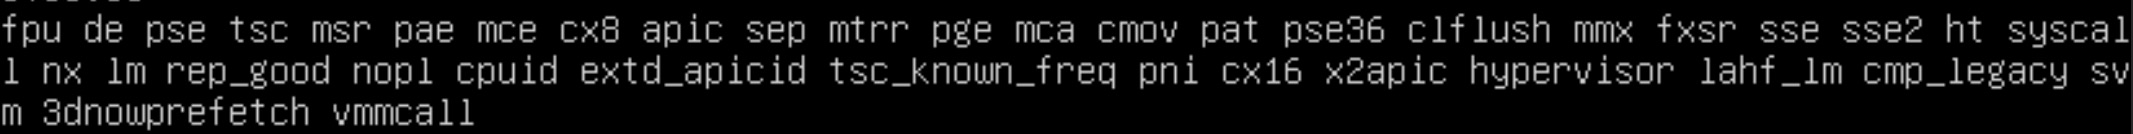
\includegraphics[width=1\textwidth]
    {assets/pics/lscpu_original.jpeg}
    \caption{Flag default KVM}
    \label{fig:lscpu_original}
\end{figure}

Terlihat pada gambar \ref{fig:lscpu_original} sama dengan Gambar \ref{fig:flag_kvm_host} di text yang ditebalkan. Dalam penelitian ini, flag yang akan diuji adalah \texttt{ssse3, sse4.1, sse4.2, sse4a, dan aes}. Semua flag SSE akan digunakan untuk percobaan kompresi video, sementara sse4.2 akan digunakan untuk validasi integritas data dengan CRC32, dan flag AES akan digunakan untuk enkripsi menggunakan AES. Harapannya, tuning ini akan memberikan peningkatan kinerja yang signifikan dibandingkan dengan konfigurasi default dari KVM.

Untuk melakukan tuning flag pada Hypervisor KVM, langkah pertama yang harus dilakukan adalah melihat daftar lengkap virtual machine yang sedang berjalan di sistem. Hal ini dapat dilakukan dengan menggunakan perintah:

\begin{listing}[H]
    \begin{minted}{bash}
    $ sudo virsh list
    \end{minted}
\end{listing}

Keluaran dari perintah ini adalah:
\begin{figure}
    \centering
    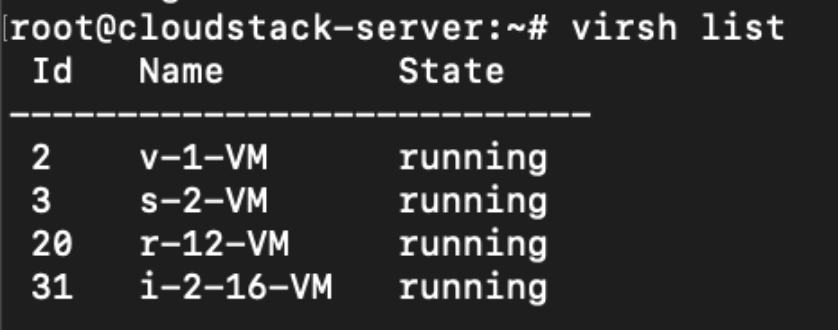
\includegraphics[width=0.5\textwidth]
    {assets/pics/virsh_list.png}
    \caption{Keluaran perintah \texttt{virsh list}}
    \label{fig:virsh_list}
\end{figure}

Pada Gambar \ref{fig:virsh_list} terlihat daftar virtual machine yang sedang berjalan di sistem. Dari daftar ini, virtual machine yang akan di-tuning adalah \texttt{i-2-16-VM}. Setelah mendapatkan nama virtual machine yang akan di-tuning (\texttt{i-2-16-VM}), gunakan perintah \texttt{virsh edit i-2-16-VM} untuk melihat konfigurasi virtual machine tersebut.

\begin{figure}
    \centering
    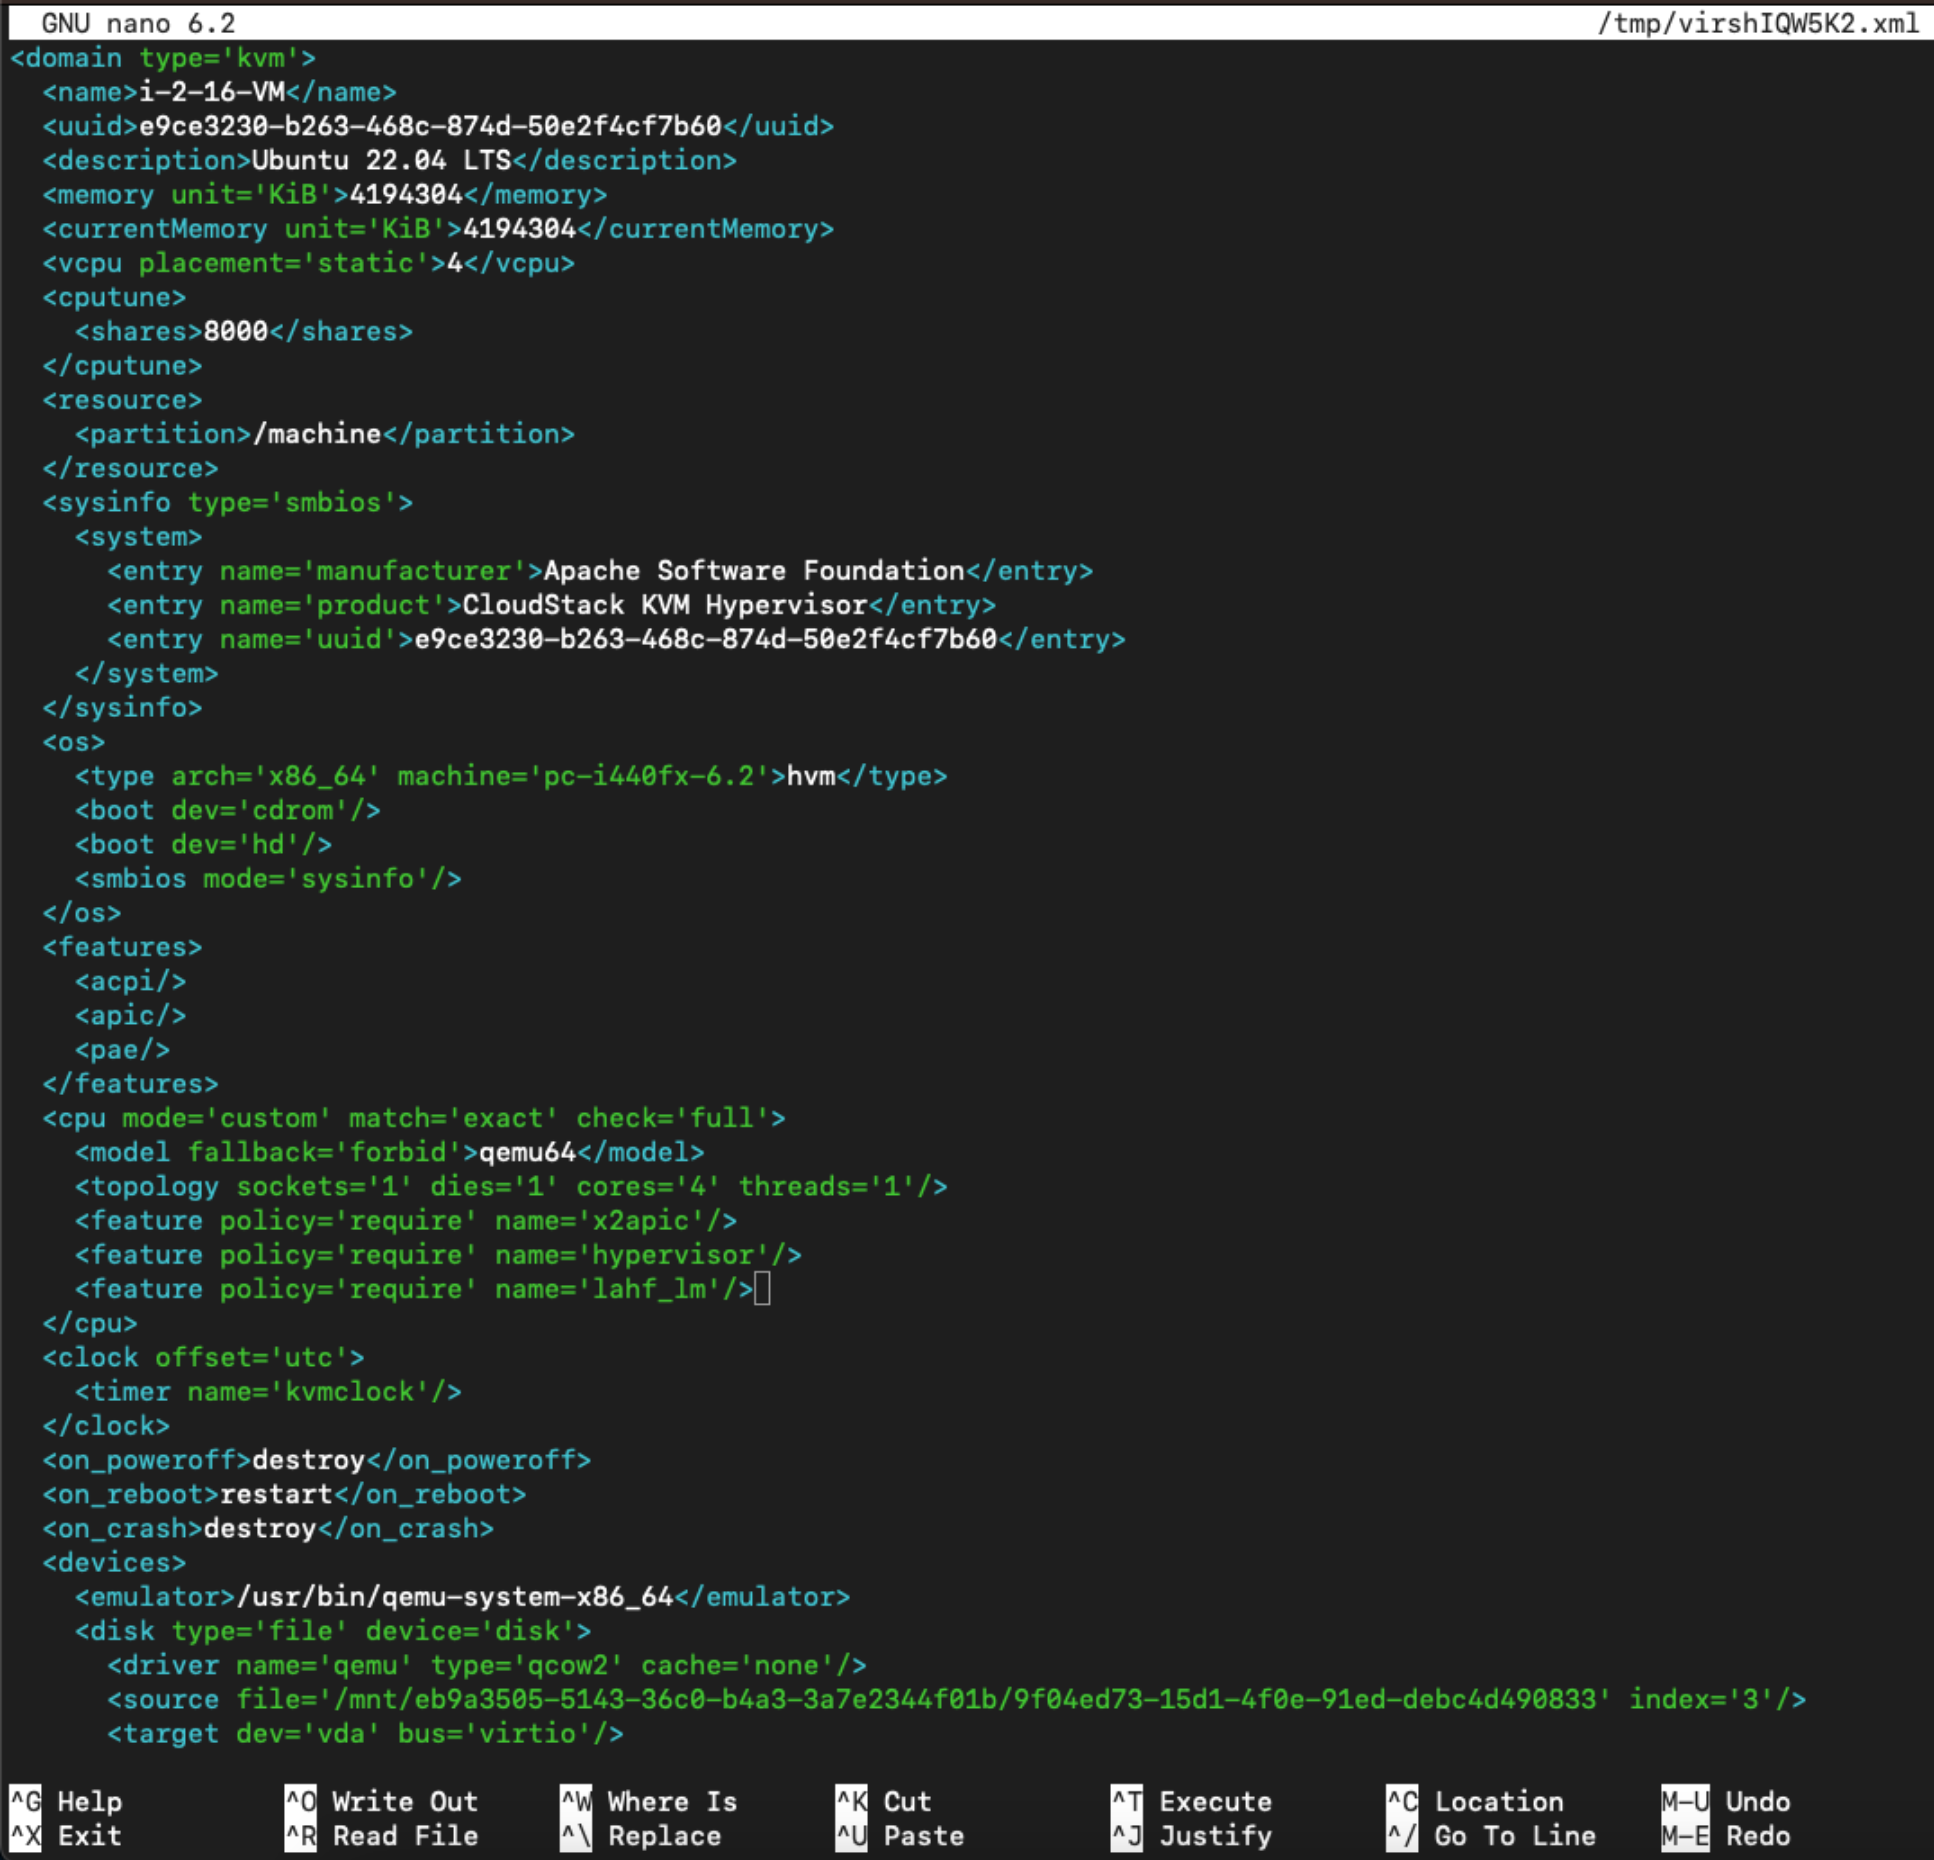
\includegraphics[width=0.9\textwidth]
    {assets/pics/virsh_edit1.png}
    \caption{Perintah \texttt{virsh edit i-2-16-VM} untuk melihat konfigurasi virtual machine \texttt{i-2-16-VM}}
    \label{fig:virsh_edit1}
\end{figure}

Pada gambar \ref{fig:virsh_edit1} terlihat konfigurasi virtual machine \texttt{i-2-16-VM}. Dari konfigurasi ini kita akan fokus pada bagian:

\begin{listing}[H]
    \begin{minted}{xml}
        ...

        <cpu mode='custom' match='exact' check='full'>
            <model fallback='forbid'>qemu64</model>
            <topology sockets='1' dies='1' cores='4' threads='1'/>
            <feature policy='require' name='x2apic'/>
            <feature policy='require' name='hypervisor'/> 
            <feature policy='require' name='lahf_1m'/>
        </cpu>
        
        ...
    \end{minted}
    \caption{Konfigurasi flag default}
    \label{code:default_kvm_xml}
\end{listing}

Kode \ref{code:default_kvm_xml} menampilkan konfigurasi flag default dari hypervisor KVM. Langkah berikutnya adalah menambahkan flag instruksi yang tidak termasuk dalam konfigurasi KVM default. Untuk melakukan ini, dilakukan duplikasi konfigurasi tersebut ke dalam sebuah file baru, seperti dalam penelitian ini yang akan disimpan di file \texttt{tuned\_kvm.xml}. Setelah disimpan di file \texttt{tuned\_kvm.xml}, selanjutnya dilakukan penambahan fitur yang diinginkan.

\begin{listing}[H]
    \begin{minted}{xml}
        ...

        <cpu mode='custom' match='exact' check='full'>
            <model fallback='forbid'>qemu64</model>
            <topology sockets='1' dies='1' cores='4' threads='1'/>
            <feature policy='require' name='x2apic'/>
            <feature policy='require' name='hypervisor'/> 
            <feature policy='require' name='lahf_1m'/>
            <feature policy='require' name='ssse3'/>
        </cpu>
        
        ...
    \end{minted}
    \caption{Konfigurasi flag ssse3}
    \label{code:ssse3_kvm_xml}
\end{listing}

Pada kode \ref{code:ssse3_kvm_xml}, fitur \texttt{ssse3} ditambahkan dengan menambahkan baris \texttt{<feature policy='require' name='ssse3'/>} pada kode tersebut. Setelah mengubah file \texttt{tuned\_kvm.xml}, \saya\ menyimpan perubahan pada file tersebut. Selanjutnya, mematikan mesin virtual dengan menggunakan perintah \texttt{destroy}:

\begin{listing}[H]
    \begin{minted}{bash}
    $ sudo virsh destroy i-2-16-VM
    \end{minted}
\end{listing}

Setelah virtual machine dimatikan, langkah selanjutnya adalah membuat virtual machine baru berdasarkan konfigurasi yang telah diubah sebelumnya. Hal ini dapat dilakukan dengan menggunakan perintah:

\begin{listing}[H]
    \begin{minted}{bash}
    $ sudo  virsh create tuned_kvm.xml
    \end{minted}
\end{listing}

Dengan perintah ini maka \vm\ \texttt{i-2-16-VM} akan dibuat menggunakan konfigurasi \texttt{tuned\_kvm.xml}. Kita dapat melihat perubahan pada \vm\ \texttt{i-2-16-VM} dengan menggunakan perintah \texttt{lscpu} pada console virtual machine.

\begin{figure}
    \centering
    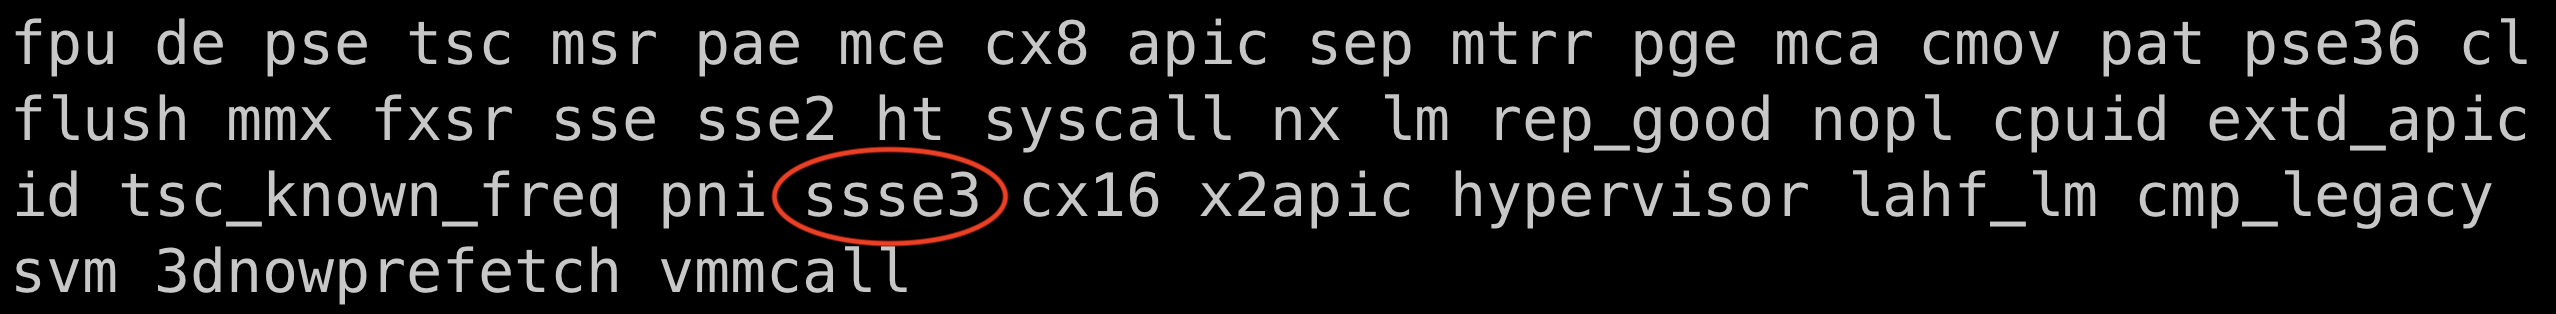
\includegraphics[width=1\textwidth]
    {assets/pics/lscpu_ssse3.jpeg}
    \caption{Flag tuned dengan ssse3}
    \label{fig:lscpu_ssse3}
\end{figure}

Dengan ini menandakan bahwa flag \texttt{ssse3} pada \vm\ \texttt{i-2-16-VM} sudah diaktifkan dan Hypervisor KVM sudah berhasil dituning.

%-----------------------------------------------------------------------------%
\subsection{Konfigurasi Hypervisor KVM untuk Kompresi Video}
%-----------------------------------------------------------------------------%
Pengujian kompresi video akan menggunakan konfigurasi seperti terlihat pada kode \ref{code:tuned_kompresi_video} yaitu dengan menggunakan flag ssse3, sse4.1, sse4.2, dan sse4a. Pemilihan flag-flag ini didasarkan pada instruksi SIMD (Single Instruction, Multiple Data) yang digunakan untuk operasi vektor pada data. Instruksi SIMD memungkinkan prosesor melakukan operasi secara bersamaan pada beberapa elemen data, sehingga mempercepat proses kompresi video dengan memanfaatkan kemampuan tersebut.

\begin{listing}[H]
    \begin{minted}{xml}
        ...

        <cpu mode='custom' match='exact' check='full'>
            <model fallback='forbid'>qemu64</model>
            <topology sockets='1' dies='1' cores='4' threads='1'/>
            <feature policy='require' name='x2apic'/>
            <feature policy='require' name='hypervisor'/> 
            <feature policy='require' name='lahf_1m'/>
            <feature policy='require' name='ssse3'/>
            <feature policy='require' name='sse4.1'/>
            <feature policy='require' name='sse4.2'/>
            <feature policy='require' name='sse4a'/>
        </cpu>
        
        ...
    \end{minted}
    \caption{Konfigurasi Hypervisor KVM untuk Kompresi Video}
    \label{code:tuned_kompresi_video}
\end{listing}

%-----------------------------------------------------------------------------%
\subsection{Konfigurasi Hypervisor KVM untuk Validasi Integritas Data}
%-----------------------------------------------------------------------------%
Untuk melakukan pengujian dengan validasi integritas data akan digunakan konfigurasi seperti pada kode \ref{code:tuned_validasi_integritas_file}. Flag yang akan digunakan adalah sse4.2. Flag ini dipilih dikarenakan salah satu kemampuan yang dimiliki oleh flag ini adalah mendukung instruksi CRC32 yang akan digunakan untuk validasi integritas data.

\begin{listing}[H]
    \begin{minted}{xml}
        ...

        <cpu mode='custom' match='exact' check='full'>
            <model fallback='forbid'>qemu64</model>
            <topology sockets='1' dies='1' cores='4' threads='1'/>
            <feature policy='require' name='x2apic'/>
            <feature policy='require' name='hypervisor'/> 
            <feature policy='require' name='lahf_1m'/>
            <feature policy='require' name='sse4.2'/>
        </cpu>
        
        ...
    \end{minted}
    \caption{Konfigurasi Hypervisor KVM untuk Validasi Integritas Data}
    \label{code:tuned_validasi_integritas_file}
\end{listing}

%-----------------------------------------------------------------------------%
\subsection{Konfigurasi Hypervisor KVM untuk Enkripsi AES}
%-----------------------------------------------------------------------------%
Untuk melakukan pengujian dengan enkripsi AES akan digunakan konfigurasi seperti pada kode \ref{code:tuned_enkripsi_aes}. Flag yang akan digunakan adalah aes. Flag ini dipilih dikarenakan salah satu kemampuan yang dimiliki oleh flag ini adalah mendukung instruksi AES yang akan digunakan untuk enkripsi AES.

\begin{listing}[H]
    \begin{minted}{xml}
        ...

        <cpu mode='custom' match='exact' check='full'>
            <model fallback='forbid'>qemu64</model>
            <topology sockets='1' dies='1' cores='4' threads='1'/>
            <feature policy='require' name='x2apic'/>
            <feature policy='require' name='hypervisor'/> 
            <feature policy='require' name='lahf_1m'/>
            <feature policy='require' name='aes'/>
        </cpu>
        
        ...
    \end{minted}
    \caption{Konfigurasi Hypervisor KVM untuk Enkripsi AES}
    \label{code:tuned_enkripsi_aes}
\end{listing}

%-----------------------------------------------------------------------------%
\section{Skenario Pengujian Tuning}
%-----------------------------------------------------------------------------%
Pada bagian ini akan dijelaskan skenario pengujian yang akan dilakukan untuk mengukur dampak tuning yang dilakukan pada Hypervisor KVM terhadap kinerja virtual machine. Pengujian akan dilakukan dengan menggunakan tiga skenario yang berbeda, yaitu kompresi video, validasi integritas data, dan enkripsi dan dekripsi AES. Setiap skenario akan dijalankan pada virtual machine yang telah dituning dengan konfigurasi yang sesuai.

%-----------------------------------------------------------------------------%
\subsection{Skenario Pengujian Kompresi Video}
%-----------------------------------------------------------------------------%
\begin{figure}
    \centering
    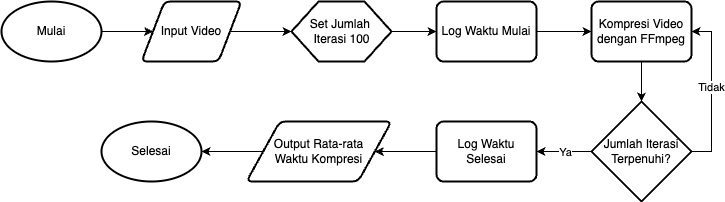
\includegraphics[width=1\textwidth]
    {assets/pics/code-flowchart/flowchart_kompresi_video.png}
    \caption{Flowchat Kode Pengujian Kompresi Video}
    \label{fig:flowchart_kompresi_video}
\end{figure}

Pada pengujian kompresi video akan dilakukan dengan menggunakan perangkat lunak ffmpeg untuk melakukan kompresi video. Flow untuk melakukan pengujian dengan kompresi video dapat terlihat di gambar \ref{fig:flowchart_kompresi_video}. Pengujian ini akan mengukur waktu yang diperlukan untuk melakukan kompresi video dengan menggunakan konfigurasi tuning yang telah dilakukan pada Hypervisor KVM. Pengujian ini akan dilakukan dengan menggunakan video yang berjudul \texttt{Times Square Day Wide} yang memiliki durasi 10 detik dan resolusi 4k. Video ini akan dikompresi menggunakan codec h265 dengan preset medium. Pengujian akan dijalankan sebanyak 100 kali per tuning dan diukur waktu yang diperlukan untuk menyelesaikan proses kompresi video. Script bash lengkap yang digunakan untuk melakukan pengujian kompresi video dapat dilihat di \textbf{kode \ref{code:kode_pengujian_kompresi_video}} pada lampiran.

%-----------------------------------------------------------------------------%
\subsection{Skenario Pengujian Validasi Integritas Data}
%-----------------------------------------------------------------------------%
\begin{figure}
    \centering
    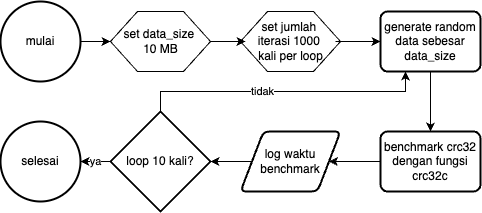
\includegraphics[width=1\textwidth]
    {assets/pics/code-flowchart/flowchart_crc32.png}
    \caption{Flowchat Kode Pengujian Validasi Integritas Data}
    \label{fig:flowchart_crc32}
\end{figure}

Pada pengujian validasi integritas data akan dilakukan dengan menggunakan library crc32c dari python untuk melakukan validasi pada sebuah data. Flow untuk melakukan pengujian validasi integritas data dapat dilihat pada gambar \ref{fig:flowchart_crc32}. Pengujian ini akan mengukur waktu yang diperlukan untuk melakukan perhitungan CRC32 pada data bytearray yang berukuran 10 MB. Pengujian ini akan dijalankan sebanyak 100 kali per tuning kemudian diukur waktu yang diperlukan untuk menyelesaikan proses perhitungan CRC32. Kode python lengkap yang digunakan untuk melakukan pengujian validasi integritas data dapat dilihat di \textbf{kode \ref{code:kode_pengujian_validasi_integritas_data}} pada lampirn.

%-----------------------------------------------------------------------------%
\subsection{Skenario Pengujian Enkripsi AES}
%-----------------------------------------------------------------------------%
\begin{figure}
    \centering
    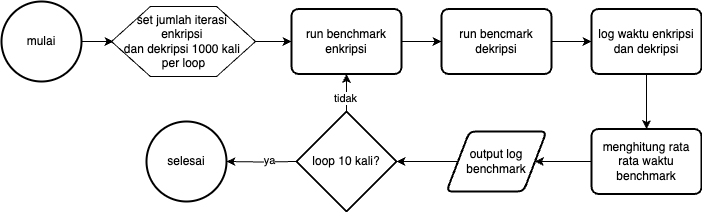
\includegraphics[width=1\textwidth]
    {assets/pics/code-flowchart/flowchart_aes.png}
    \caption{Flowchat Kode Pengujian Enkripsi dan Dekripsi AES}
    \label{fig:flowchart_aes}
\end{figure}

Pada pengujian enkripsi AES akan dilakukan dengan menggunakan library cryptography dari python untuk melakukan enkripsi AES. Flow untuk melakukan pengujian dengan enkripsi dan dekripsi AES dapat dilihat pada gambar \ref{fig:flowchart_aes} Pengujian ini akan mengukur waktu yang diperlukan untuk melakukan enkripsi AES pada data teks yang dapat dilihat pada Gambar \ref{fig:aesPlaintextData}. Pengujian ini akan dijalankan sebanyak 100 kali per tuning dan diukur waktu yang diperlukan untuk menyelesaikan proses enkripsi dan dekripsi AES. Kode python yang digunakan untuk melakukan pengujian enkripsi AES dapat dilihat di \textbf{kode \ref{code:pengujian_enkripsi_aes}} pada lampiran.

%-----------------------------------------------------------------------------%
\section{Skenario Analisis}
%-----------------------------------------------------------------------------%
Analisis akan dilakukan dengan melakukan perhitungan menggunakan formula \texttt{speedup}. Diasumsikan bahwa T(1) adalah waktu eksekusi Test dengan konfigurasi default, dan T(p) adalah waktu eksekusi Test dengan konfigurasi yang telah dituning \cite{beuwolfCetin}.

Formula \texttt{speedup} dinyatakan sebagai berikut:

\begin{equation}
    S(p) = \frac{T(1)}{T(p)}
    \label{eq:formula}
\end{equation}

Berdasarkan rumus \ref{eq:formula}, jika nilai S(p) semakin besar, maka konfigurasi yang dituning semakin bagus. Hal ini menandakan bahwa tuning Hypervisor dapat mempercepat proses yang dilakukan. Sebaliknya, jika S(p) semakin kecil, maka konfigurasi yang dituning semakin lambat. Jika nilai S(p) sama, maka efek dari konfigurasi yang dituning sama dengan konfigurasi default.

Dalam analisis pengujian dengan kompresi video, \saya\ akan membandingkan waktu eksekusi antara konfigurasi Hypervisor yang tidak dituning (default) dan konfigurasi yang telah dituning. Perbandingan ini akan dilakukan dengan menggunakan formula \texttt{speedup}. Konfigurasi yang optimal adalah konfigurasi yang memiliki nilai \texttt{speedup} tertinggi, yang menunjukkan peningkatan kinerja yang signifikan dalam proses kompresi video.

Untuk analisis pengujian validasi integritas data, \saya\ akan menggunakan pendekatan yang serupa dengan analisis kompresi video. Akan dibandingkan waktu eksekusi antara konfigurasi Hypervisor yang tidak dituning (default) dan konfigurasi yang telah dituning menggunakan formula \texttt{speedup}. Nilai S(p) yang lebih besar menunjukkan bahwa konfigurasi yang dituning lebih efisien dalam memverifikasi integritas data dibandingkan dengan konfigurasi default.

Dalam analisis pengujian enkripsi AES, \saya\ akan menggunakan metode yang sama seperti analisis sebelumnya, yaitu dengan membandingkan waktu eksekusi antara konfigurasi Hypervisor yang tidak dituning (default) dan konfigurasi yang telah dituning menggunakan formula \texttt{speedup}. Nilai S(p) yang lebih besar menunjukkan bahwa konfigurasi yang dituning lebih efisien dalam melakukan enkripsi AES dibandingkan dengan konfigurasi default.

Dengan menganalisis nilai \texttt{speedup}, penulis dapat mengevaluasi dan membandingkan kinerja berbagai konfigurasi Hypervisor dalam melakukan tugas-tugas seperti kompresi video, validasi integritas data, dan enkripsi AES. Konfigurasi dengan nilai \texttt{speedup} tertinggi akan menjadi pilihan yang optimal untuk meningkatkan kinerja dan efisiensi dalam setiap tugas yang diuji.